
%(BEGIN_QUESTION)
% Copyright 2008, Tony R. Kuphaldt, released under the Creative Commons Attribution License (v 1.0)
% This means you may do almost anything with this work of mine, so long as you give me proper credit

The driver (output) circuits inside of EIA/TIA-485 transceivers must be equipped with {\it tri-state} outputs.  Explain what a ``tri-state'' output is, and why it is essential for multipoint transceivers to have:

$$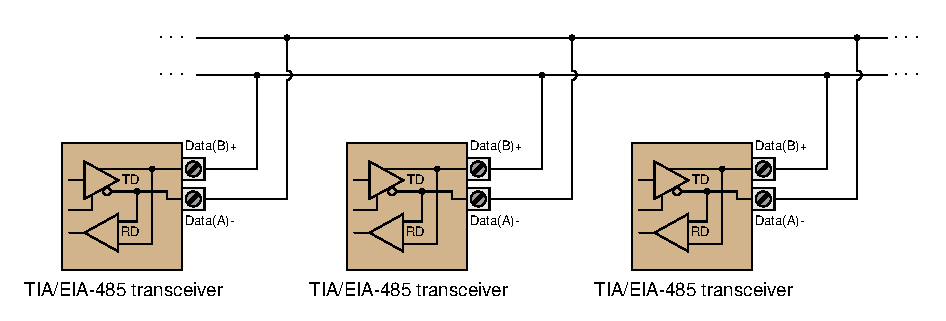
\includegraphics[width=15.5cm]{i02199x01.eps}$$

Also, would you classify the above network as a {\it simplex}, {\it half-duplex}, or {\it full-duplex} system?  Explain why.

\vskip 20pt \vbox{\hrule \hbox{\strut \vrule{} {\bf Suggestions for Socratic discussion} \vrule} \hrule}

\begin{itemize}
\item{} Can you identify the channel arbitration strategy (e.g master-slave, token passing, TDMA) of this digital network from its schematic diagram? If so, which strategy do you think it uses?
\item{} Does this digital network require termination resistors?  If so, where should they be placed?
\end{itemize}

\underbar{file i02199}
%(END_QUESTION)





%(BEGIN_ANSWER)

A tri-state digital device has three output modes: {\it high}, {\it low}, and {\it high-Z}, the latter state being where the output transistors all go into cutoff and ``disconnect'' themselves so they neither source nor sink current.

\vskip 10pt

Does this symbol jog some memories of your previous electronics studies?

$$\includegraphics[width=15.5cm]{i02199x02.eps}$$

%(END_ANSWER)





%(BEGIN_NOTES)

This is a half-duplex system, where tri-state buffers are necessary so that no receiving devices attempt to force a state on the lines.  All receiving devices must switch their drivers to ``high-impedance'' mode and let the one transmitting device define the line's mark and space states.

\vskip 10pt

A common conceptual barrier among electronics students seems to be understanding why it is bad to have multiple logic gate outputs connected together (paralleled).  This is a good opportunity to review this important, yet easily misunderstood, topic.

\vskip 10pt

Of course, simplex communication is possible here too, if only one driver is ever allowed to transmit!

\vfil \eject

\noindent
{\bf Summary Quiz:}

{\it Tri-state driver} circuits are essential for digital devices to work within any {\it multipoint} network.  Identify the consequence of digital devices {\it not} having tri-state circuits in a multipoint network:

\begin{itemize}
\item{} Only one device could communicate at a time
\vskip 5pt 
\item{} Power consumption would be excessive
\vskip 5pt 
\item{} High-speed communication would be impossible
\vskip 5pt 
\item{} Multiple device output states would conflict
\vskip 5pt 
\item{} An electrical shock hazard may result 
\vskip 5pt 
\item{} The devices might burst into flames!
\end{itemize}


%INDEX% Electronics review: tri-state output
%INDEX% Networking, multipoint: EIA/TIA-485

%(END_NOTES)


